%!Mode:: "TeX:UTF-8"
%!TEX TS-program = xelatex
\documentclass{ctexart}
\newif\ifpreface
%\prefacetrue
\usepackage{fontspec}
\usepackage{bbm}
\usepackage{tikz}
\usepackage{amsmath,amssymb,amsthm,color,mathrsfs}
\usepackage{fixdif}
\usepackage{hyperref}
\usepackage{cleveref}
\usepackage{enumitem}%
\usepackage{expl3}
\usepackage{lipsum}
\usepackage[margin=0pt]{geometry}
\usepackage{listings}
\definecolor{mGreen}{rgb}{0,0.6,0}
\definecolor{mGray}{rgb}{0.5,0.5,0.5}
\definecolor{mPurple}{rgb}{0.58,0,0.82}
\definecolor{backgroundColour}{rgb}{0.95,0.95,0.92}

\lstdefinestyle{CStyle}{
  backgroundcolor=\color{backgroundColour},
  commentstyle=\color{mGreen},
  keywordstyle=\color{magenta},
  numberstyle=\tiny\color{mGray},
  stringstyle=\color{mPurple},
  basicstyle=\footnotesize,
  breakatwhitespace=false,
  breaklines=true,
  captionpos=b,
  keepspaces=true,
  numbers=left,
  numbersep=5pt,
  showspaces=false,
  showstringspaces=false,
  showtabs=false,
  tabsize=2,
  language=C
}
\usetikzlibrary{calc}
\theoremstyle{remark}
\newtheorem{lemma}{Lemma}
\usepackage{fontawesome5}
\usepackage{xcolor}
\newcounter{problem}
\newcommand{\Problem}{\begin{tikzpicture}[baseline]%
    \node at (-0.02em,0.3em) {$\mathbb{P}$};%
    \node[scale=0.7] at (0.2em,-0.0em) {R};%
    \node[scale=0.7] at (0.6em,0.4em) {O};%
    \node[scale=0.8] at (1.05em,0.25em) {B};%
    \node at (1.55em,0.3em) {L};%
    \node[scale=0.7] at (1.75em,0.45em) {E};%
    \node at (2.35em,0.3em) {M};%
  \end{tikzpicture}%
}
\renewcommand{\theproblem}{\Roman{problem}}
\newenvironment{problem}{\refstepcounter{problem}\noindent\color{blue}\Problem\theproblem}{}

\crefname{problem}{\protect\Problem}{Problem}
\newcommand\Solution{\begin{tikzpicture}[baseline]%
    \node at (-0.04em,0.3em) {$\mathbb{S}$};%
    \node[scale=0.7] at (0.35em,0.4em) {O};%
    \node at (0.7em,0.3em) {\textit{L}};%
    \node[scale=0.7] at (0.95em,0.4em) {U};%
    \node[scale=1.1] at (1.19em,0.32em){T};%
    \node[scale=0.85] at (1.4em,0.24em){I};%
    \node at (1.9em,0.32em){$\mathcal{O}$};%
    \node[scale=0.75] at (2.3em,0.21em){\texttt{N}};%
  \end{tikzpicture}}
\newenvironment{solution}{\begin{proof}[\Solution]}{\end{proof}}
\title{\input{../../.subject}\input{../.number}}
\makeatletter
\newcommand\email[1]{\def\@email{#1}\def\@refemail{mailto:#1}}
\newcommand\schoolid[1]{\def\@schoolid{#1}}
\ifpreface
  \def\@maketitle{
  \raggedright
  {\Huge \bfseries \sffamily \@title }\\[1cm]
  {\Huge  \bfseries \sffamily\heiti\@author}\\[1cm]
  {\Huge \@schoolid}\\[1cm]
  {\Huge\href\@refemail\@email}\\[0.5cm]
  \Huge\@date\\[1cm]}
\else
  \def\@maketitle{
    \raggedright
    \begin{center}
      {\Huge \bfseries \sffamily \@title }\\[4ex]
      {\Large  \@author}\\[4ex]
      {\large \@schoolid}\\[4ex]
      {\href\@refemail\@email}\\[4ex]
      \@date\\[8ex]
    \end{center}}
\fi
\makeatother
\ifpreface
  \usepackage[placement=bottom,scale=1,opacity=1]{background}
\fi

\author{白永乐}
\schoolid{202011150087}
\email{202011150087@mail.bnu.edu.cn}

\def\to{\rightarrow}
\newcommand{\xor}{\vee}
\newcommand{\bor}{\bigvee}
\newcommand{\band}{\bigwedge}
\newcommand{\xand}{\wedge}
\newcommand{\minus}{\mathbin{\backslash}}
\newcommand{\mi}[1]{\mathscr{P}(#1)}
\newcommand{\card}{\mathrm{card}}
\newcommand{\oto}{\leftrightarrow}
\newcommand{\hin}{\hat{\in}}
\newcommand{\gl}{\mathrm{GL}}
\newcommand{\im}{\mathrm{Im}}
\newcommand{\re }{\mathrm{Re }}
\newcommand{\rank}{\mathrm{rank}}
\newcommand{\tra}{\mathop{\mathrm{tr}}}
\renewcommand{\char}{\mathop{\mathrm{char}}}
\DeclareMathOperator{\ot}{ordertype}
\DeclareMathOperator{\dom}{dom}
\DeclareMathOperator{\ran}{ran}

\begin{document}
\large
\iffalse
  \setlength{\baselineskip}{1.2em}
  \ifpreface
    \backgroundsetup{contents={%
    \begin{tikzpicture}
      \fill [white] (current page.north west) rectangle ($(current page.north east)!.3!(current page.south east)$) coordinate (a);
      \fill [bgc] (current page.south west) rectangle (a);
\end{tikzpicture}}}
\definecolor{word}{rgb}{1,1,0}
\definecolor{bgc}{rgb}{1,0.95,0}
\setlength{\parindent}{0pt}
\thispagestyle{empty}
\begin{tikzpicture}%
  % \node[xscale=2,yscale=4] at (0cm,0cm) {\sffamily\bfseries \color{word} under};%
  \node[xscale=4.5,yscale=10] at (10cm,1cm) {\sffamily\bfseries \color{word} Graduate Homework};%
  \node[xscale=4.5,yscale=10] at (8cm,-2.5cm) {\sffamily\bfseries \color{word} In Mathematics};%
\end{tikzpicture}
\ \vspace{1cm}\\
\begin{minipage}{0.25\textwidth}
  \textcolor{bgc}{王胤雅是傻逼}
\end{minipage}
\begin{minipage}{0.75\textwidth}
  \maketitle
\end{minipage}
\vspace{4cm}\ \\
\begin{minipage}{0.2\textwidth}
  \
\end{minipage}
\begin{minipage}{0.8\textwidth}
  {\Huge
    \textinconsolatanf{}
  }General fire extinguisher
\end{minipage}
\newpage\backgroundsetup{contents={}}\setlength{\parindent}{2em}

  \else
    \maketitle
  \fi
\fi
\newgeometry{left=2cm,right=2cm,top=2cm,bottom=2cm}
%from_here_to_type

\begin{problem}\label{pro:1}
  Assume \(A=\{a \in P \mid a \mid m\} = \{q_i \mid i=1,\cdots,s\}\), where \(P \subset \mathbb{N}\), \(\forall p \in P\), \(p\) is prime,
  \(s = |A|\).
  Prove: \(g\) is the primative root mod \(m\) \(\iff\)
  \(g\) is \(q_i\)-tic non-residue mod \(m\), \(\forall i=1,\cdots,s\).
\end{problem}
\begin{solution}
  On one hand, assume \(g\) is \(q_i\)-th power residue of \(m\), then \(g \equiv h^{q_i} \mod m\).
  So \(g^{\frac{\phi(m)}{q_i}}\equiv h^{\phi(m)}\equiv 1 \mod m\), contradiction!

  On the other hand, assume \(o(g)<\phi(m)\). Easily \(o(g) \mid \phi(m)\), so \(\frac{\phi(m)}{o(g)} \in \mathbb{Z}\).
  So \(\exists i,q_i \mid \frac{\phi(m)}{o(g)}\). Then \(g^{\frac{\phi(m)}{q_i}} \equiv 1 \mod m\).
  Then \(g\) is \(q_i\)-th power residue of \(m\).
\end{solution}
\begin{problem}\label{pro:2}
  Prove:
  \begin{enumerate}
    \item \(10\) is the primative root mod \(17,257\).
    \item The length of repetend of \(\frac{1}{17}\) is \(16\), the length of repetend of \(\frac{1}{257}\) is \(256\).
  \end{enumerate}
\end{problem}
\begin{solution}
  Easily \(\phi(17)=16=2^4\). So we only need to check \(10^8 \not \equiv 1 \mod 17\).
  Easily \(10^8 \equiv 100^4 \equiv (-2)^4 \equiv 2^4 \equiv -1 \mod 17\).
  So \(10\) is primative root of \(17\).

  Easily \(\phi(257)=256=2^8\), so we only need to check \(10^{128} \not \equiv 1 \mod 257\).
  By calculation easily to get that \(10^{128}\equiv -1 \mod 257\).
  So \(10\) is primative root of \(17\).

  Since \(10\) is primative root of \(17,257\), we know the length of loop-body of \(\frac{1}{17},\frac{1}{257}\) are \(16,256\).
\end{solution}
\begin{problem}\label{pro:3}
  Apply index table to solve the equation \[
    x^{15 } \equiv 14 \pmod{41}.
  \]
\end{problem}
\begin{solution}
  Use \(6\) as primative root of \(41\), we have this table of index:
  \begin{figure}
    \centering
    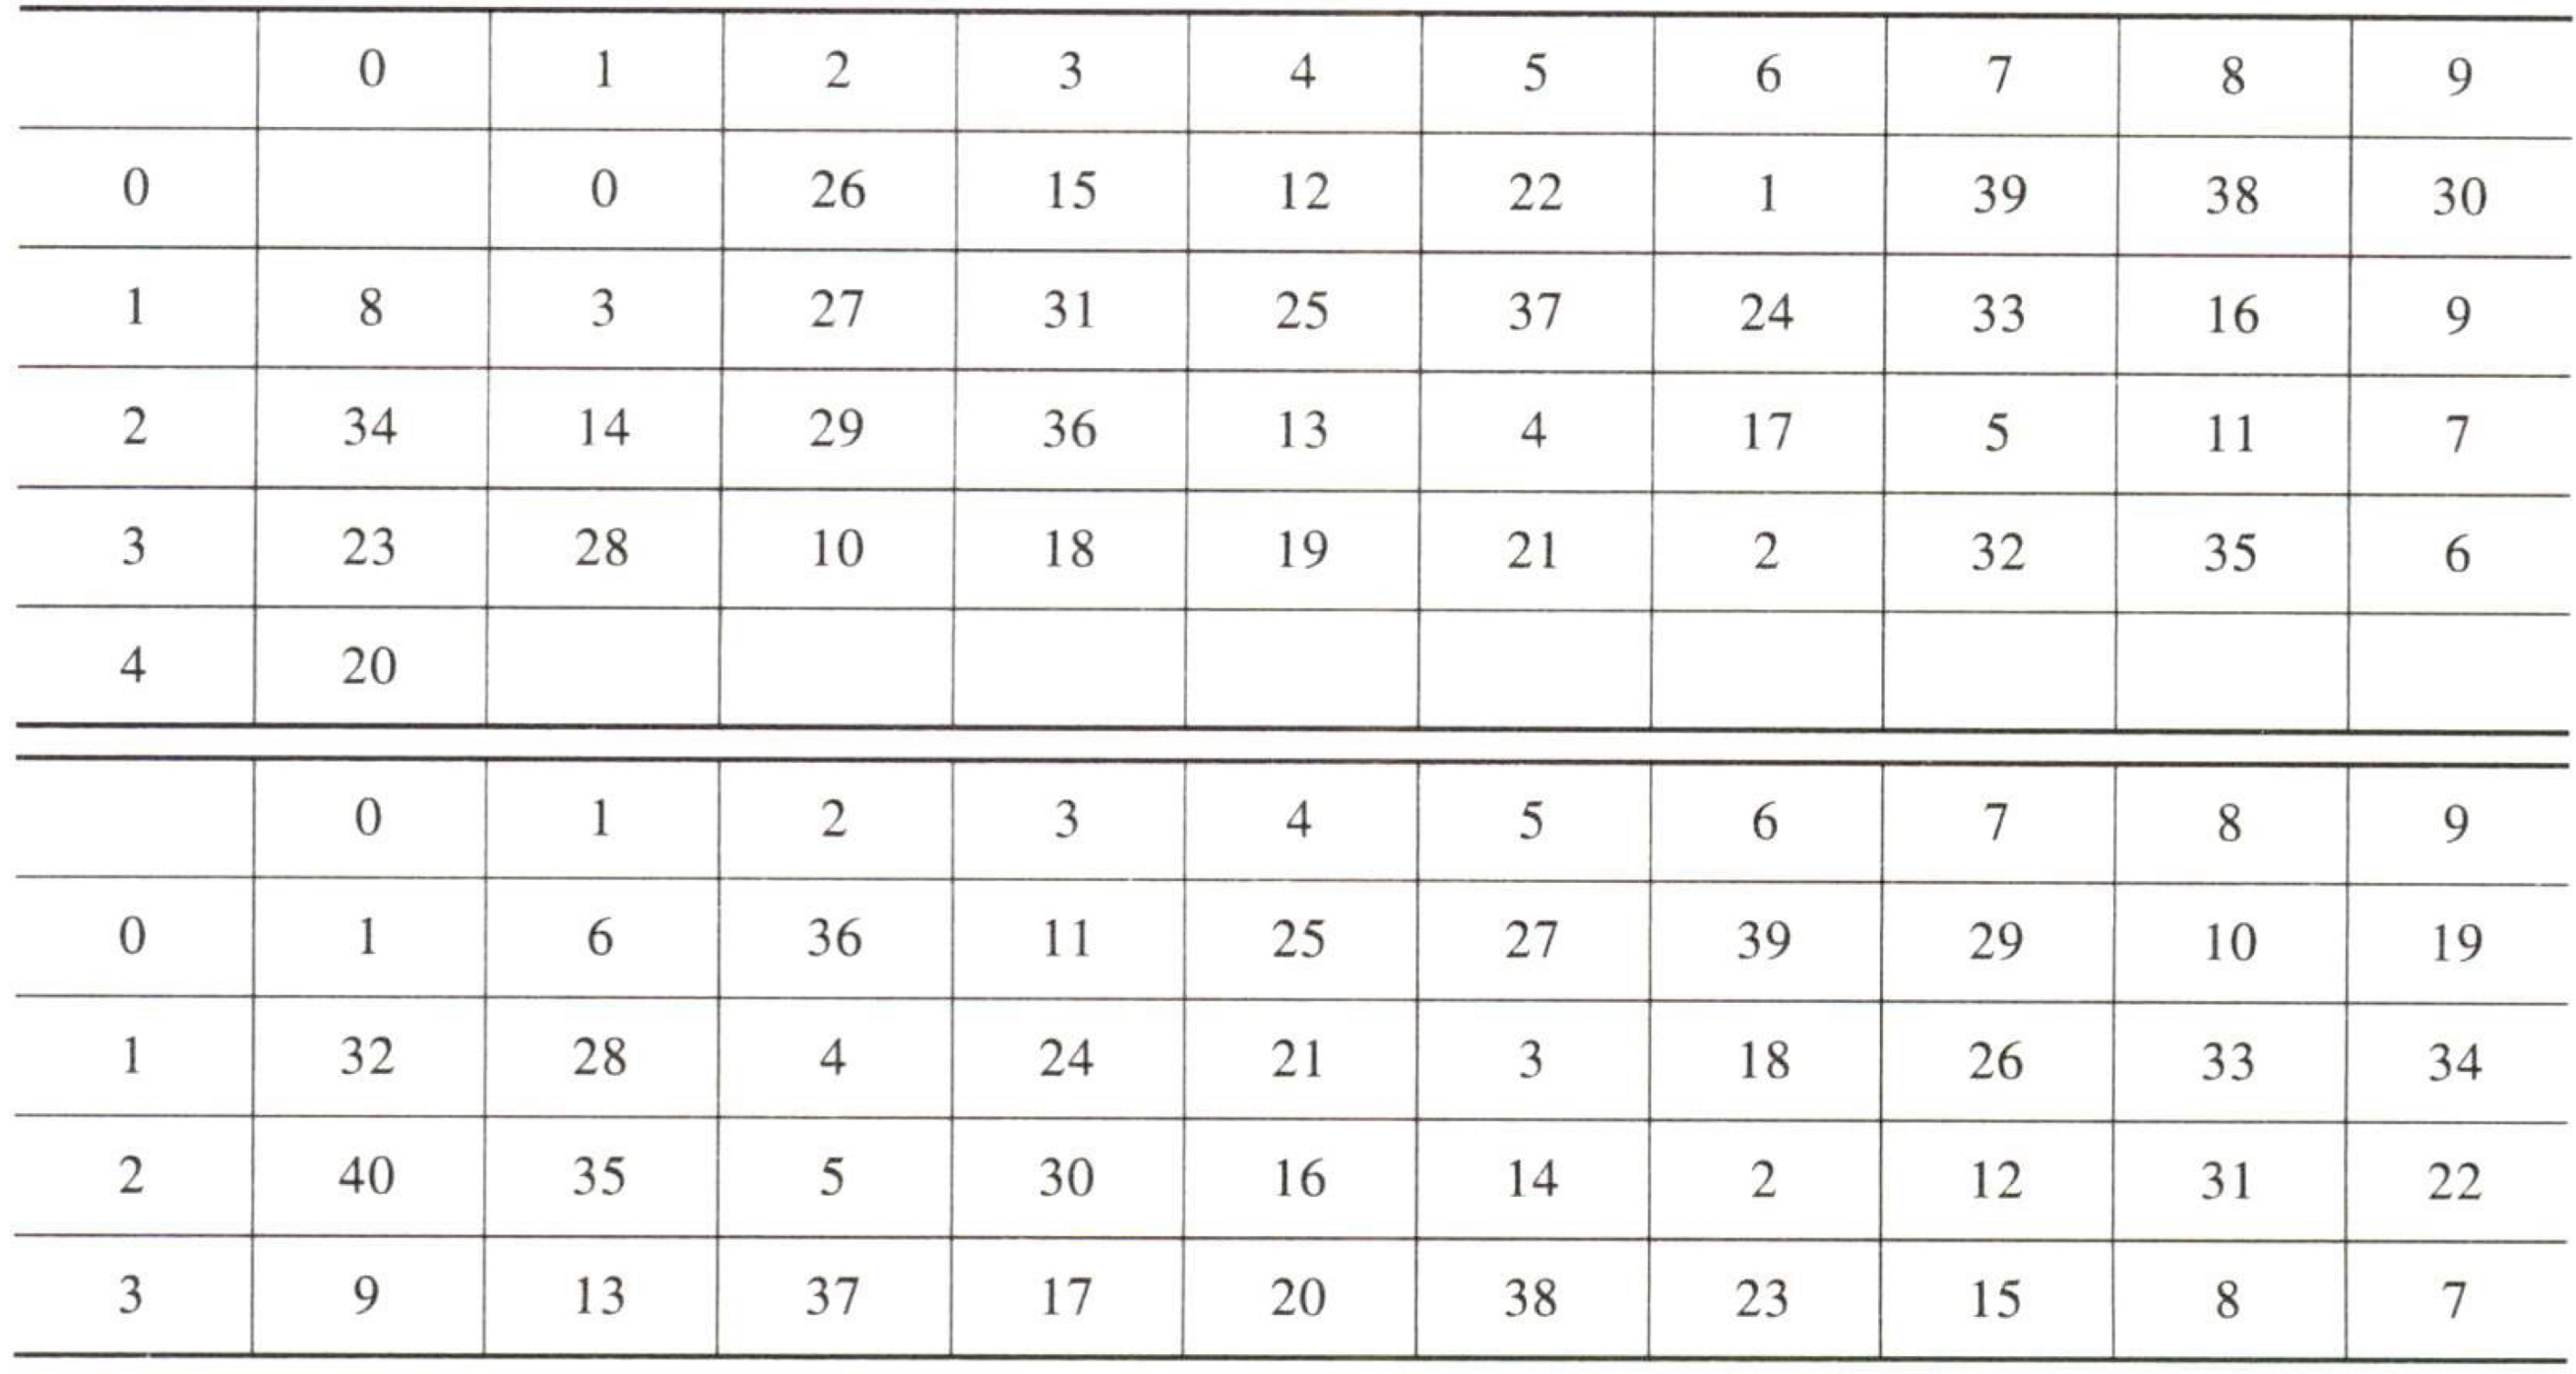
\includegraphics[width=\linewidth]{./mod41.png}
  \end{figure}
  Then \(x^{15} \equiv 14 \mod 41 \iff 15 \ind x \equiv \ind 14 \mod 40 \iff 3 \ind x \equiv 5 \mod 8 \iff \ind x \equiv 7 \mod 8\).
  So \(\ind x = 7,15,22,29,36\). So \(x \equiv 29,3,5,22,23 \mod 41\).
\end{solution}
\begin{problem}\label{pro:4}
  Assume \(m >2\) has primative root, prove for any primative root \(g\) of \(m\), we have \(\ind_g -1=\frac{1}{2}\phi(m)\).
\end{problem}
\begin{solution}
  We have \(g^{\phi(m)} \equiv 1 \mod m\).
  So \(\ind_g 1=0\).
  Since \((-1)^2 \equiv 1 \mod m\), we have \(2 \ind_g -1 \equiv \ind_g 1 \mod \phi(m)\).
  So \(\ind_g -1 \equiv 0 \mod \frac{\phi(m)}{2}\).
  But obviously \(\ind_g -1 \neq 0\), so we obtain \(\ind_g -1 = \frac{\phi(m)}{2}\).
\end{solution}

\begin{problem}\label{pro:5}
  Assume \(g_1,g_2\) are two primative root mod \(m\), prove:
  \begin{enumerate}
    \item \(\ind_{g_1}g \cdot \ind_{g}g_1 \equiv 1 \pmod{\phi(m)}\);
    \item \(\ind_g a \equiv \ind_g g_1 \cdot\ind_{g_1}a \pmod{\phi(m)}\)
  \end{enumerate}
\end{problem}
\begin{solution}
  \begin{enumerate}
    \item Let \(a=\ind_{g_1}g,b=\ind_{g}g_1\).
      By the defination, we can get that \(g_1^a \equiv g \pmod{\phi(m)}, g^b \equiv g_1 \pmod{\phi(m)}\).
      Then \((g_1^{a})^b = g_1^{ab}\equiv g^b \equiv g_1 \pmod{\phi(m)}\).
      Since \(g_1\) is the primative root of \(m\), then \(ab \equiv 1 \pmod{\phi(m)}\).
    \item Only need to check \(g^{\ind_g g_1 \cdot \ind_{g_1} a} \equiv a \mod m\).
      Easily \(g^{\ind_g g_1 \cdot \ind_{g_1} a} \equiv g_1^{\ind_{g_1} a}\equiv a \mod m \).
  \end{enumerate}
\end{solution}

\end{document}
